%----------------------------------------------------------------------------------------
% Preambulo y Configuración
%----------------------------------------------------------------------------------------

\documentclass[
    11pt,
    spanish,
    singlespacing,
    parskip,
    headsepline,
    bookmarks=true,
    unicode=true,
    pdftoolbar=true,
    pdfmenubar=true,
    pdffitwindow=false,
    colorlinks=true,
    linkcolor=blue,
    citecolor=blue,
    urlcolor=blue
]{MastersDoctoralThesis}

\usepackage[utf8]{inputenc} % Codificación de entrada UTF-8
\usepackage[T1]{fontenc}    % Codificación de salida para caracteres especiales
\usepackage{graphicx}       % Manejo de gráficos
\usepackage{eso-pic}        % Permite agregar fondos
\usepackage{hyperref}       % Manejo de hipervínculos y marcadores

% Redefinición de caracteres problemáticos en marcadores
\hypersetup{
    pdftitle={Detección de patologías cardiopulmonares mediante redes neuronales aplicadas a señales de auscultación},
    pdfauthor={Santiago Federico Bettig},
    pdfkeywords={auscultación, sonidos cardíacos, sonidos pulmonares, aprendizaje profundo, redes neuronales convolucionales},
    pdfstartview={FitH},
    unicode=true,
    colorlinks=true,
    linkcolor=blue,
    citecolor=blue,
    urlcolor=blue
}

\pdfstringdefDisableCommands{%
  \def\texttt#1{#1}%
  \def\textbf#1{#1}%
  \def\textit#1{#1}%
  \def\"{\"}%
  \def\~{~}%
  \def\'{'}%
  \def\^{}%
  \def\textunderscore{\_} % Manejo del subrayado en marcadores
}


% Definir comandos requeridos por la clase
\newcommand{\degreename}{Especialización en Inteligencia Artificial}
\newcommand{\univname}{Universidad de Buenos Aires}
\newcommand{\keywordnames}{Palabras clave:}

% Comandos para separar el formato del contenido (antes definidos en Chapter1.tex)
\newcommand{\keyword}[1]{\textbf{#1}}
\newcommand{\tabhead}[1]{\textbf{#1}}
\newcommand{\code}[1]{\texttt{#1}}
\newcommand{\file}[1]{\texttt{\bfseries#1}}
\newcommand{\option}[1]{\texttt{\itshape#1}}
\newcommand{\grados}{$^{\circ}$}
%----------------------------------------------------------------------------------------
% Documento Principal
%----------------------------------------------------------------------------------------

\begin{document}

% Configuración de la portada
\posgrado{Carrera de Especialización en Inteligencia Artificial}
\keywords{auscultación, sonidos cardíacos, sonidos pulmonares, aprendizaje profundo, redes neuronales convolucionales}

% Incluir la portada desde un archivo separado
%----------------------------------------------------------------------------------------
% PORTADA
%----------------------------------------------------------------------------------------
\begin{titlepage}
    % Fondo completo con el PDF que incluye la barra y el logo
    \AddToShipoutPictureBG*{
\includegraphics[width=\paperwidth, height=\paperheight]{Figures/fondo.pdf}}

    % Contenido principal
    \begin{flushright}
        \setlength{\rightskip}{-2cm} % Ajusta la sangría derecha
        \vspace*{7.5cm} % Ajustar según la posición vertical deseada

        % Título
        {\fontfamily{phv}\bfseries\fontsize{30pt}{40pt}\selectfont
        Detección de patologías cardiopulmonares mediante redes neuronales aplicadas a señales de auscultación} \\[1.5cm]

        % Autor
        {\fontfamily{phv}\fontsize{20pt}{25pt}\selectfont
        Ing. Santiago Federico Bettig} \\[1cm]

        % Carrera o Maestría (comentar o descomentar la línea correspondiente)
        {\fontfamily{phv}\fontsize{15pt}{20pt}\selectfont
        % \textbf{Carrera de Especialización en Sistemas Embebidos}
        % \textbf{Carrera de Especialización en Internet de las Cosas} \\
        \textbf{Carrera de Especialización en Inteligencia Artificial}
        % \textbf{Maestría en Sistemas Embebidos} \\
        % \textbf{Maestría en Internet de las Cosas} \\
        % \textbf{Maestría en Inteligencia Artificial Embebida} \\
        % \textbf{Maestría en Computación de Borde} \\
        % \textbf{Maestría en Inteligencia Artificial} \\
        } \\[2cm]

        % Director
        {\fontfamily{phv}\fontsize{11pt}{15pt}\selectfont
        \textbf{Director:} Dr. Ing. Leandro Javier Cymberknop (CIBIO, UTN FRBA)} \\[1cm]

        % Jurados
        {\fontfamily{phv}\fontsize{11pt}{15pt}\selectfont
        \textbf{Jurados:}} \\[0.5cm]
        {\fontfamily{phv}\fontsize{11pt}{15pt}\selectfont
        Jurado 1 (pertenencia)} \\ 
        {\fontfamily{phv}\fontsize{11pt}{15pt}\selectfont
        Jurado 2 (pertenencia)} \\ 
        {\fontfamily{phv}\fontsize{11pt}{15pt}\selectfont
        Jurado 3 (pertenencia)} \\[2cm]

        % Fecha y lugar
        {\fontfamily{phv}\itshape\fontsize{10pt}{12pt}\selectfont
        Ciudad de Buenos Aires, mayo de 2027} % Ejemplo: Ciudad de Córdoba, junio de 2025
    \end{flushright}
\end{titlepage}


% Configuración del contenido preliminar
\frontmatter % Usar numeración romana para las páginas preliminares
\pagestyle{plain} % Estilo de encabezado simple

%----------------------------------------------------------------------------------------
% Resumen
%----------------------------------------------------------------------------------------

\begin{abstract}
\addchaptertocentry{\abstractname} % Agregar resumen al índice
En esta memoria se presenta el desarrollo de un sistema de clasificación automática de sonidos de auscultación cardíaca y pulmonar basado en redes neuronales, concebido como herramienta de apoyo al diagnóstico para el médico generalista. El sistema procesa grabaciones obtenidas con estetoscopios digitales, las transforma en representaciones tiempo-frecuencia y detecta la presencia de hallazgos patológicos en ambos tipos de sonido. A diferencia de la mayoría de los trabajos previos que tratan los sonidos cardíacos y pulmonares por separado, el trabajo aborda la auscultación cardiopulmonar de forma integrada y compara este enfoque con el de modelos independientes para cada órgano. El trabajo se realizó en colaboración con el Centro de Investigación y Desarrollo en Ingeniería Biomédica de la Universidad Tecnológica Nacional.

A lo largo de la memoria se describen las bases de datos utilizadas, el preprocesamiento de las señales, el diseño y el entrenamiento de los modelos, y los ensayos realizados para evaluar su desempeño. En el desarrollo se aplicaron contenidos de la especialización vinculados con el análisis de datos, el aprendizaje automático, el aprendizaje profundo, las redes neuronales convolucionales y la gestión de proyectos.
\end{abstract}

%----------------------------------------------------------------------------------------
% Agradecimientos
%----------------------------------------------------------------------------------------

\begin{acknowledgements}
\vspace{1.5cm}
Esta sección es para agradecimientos personales y es totalmente \textbf{OPCIONAL}.
\end{acknowledgements}

%----------------------------------------------------------------------------------------
% Índice
%----------------------------------------------------------------------------------------

\tableofcontents
\listoffigures
\listoftables

%----------------------------------------------------------------------------------------
% Dedicatoria
%----------------------------------------------------------------------------------------

\dedicatory{\textbf{Dedicado a... [OPCIONAL]}}

%----------------------------------------------------------------------------------------
% Capítulos
%----------------------------------------------------------------------------------------

\mainmatter % Iniciar numeración numérica para el contenido principal
\pagestyle{thesis} % Estilo de encabezado de tesis

% Incluir capítulos desde archivos separados
% Chapter 1

\chapter{Introducción general} % Main chapter title

\label{Chapter1} % For referencing the chapter elsewhere, use \ref{Chapter1}
\label{IntroGeneral}

En este capítulo se presenta el área en la que se enmarca el trabajo, el contexto y la motivación que le dieron origen, una revisión del estado del arte en la clasificación automática de sonidos de auscultación y los objetivos y el alcance del proyecto.

%----------------------------------------------------------------------------------------

\section{La auscultación cardiopulmonar}
\label{sec:auscultacion}

La auscultación es la técnica de exploración clínica que consiste en escuchar los sonidos generados en el interior del cuerpo, principalmente los del corazón y los pulmones. Desde que René Laënnec inventó el estetoscopio en 1816 y lo utilizó para vincular los sonidos torácicos con los hallazgos de autopsia \citep{roguin2006laennec}, la auscultación se convirtió en uno de los pilares del examen físico. Su vigencia se explica por tres características: es no invasiva, tiene un costo muy bajo y brinda información inmediata en el lugar de atención.

Los sonidos cardíacos normales se originan principalmente en el cierre de las válvulas y se perciben como dos golpes breves por ciclo, conocidos como primer y segundo ruido (S1 y S2). Distintas alteraciones modifican este patrón. Los soplos son sonidos producidos por el flujo turbulento de la sangre y se asocian, por ejemplo, a valvulopatías o a cardiopatías congénitas. También pueden aparecer ruidos adicionales, como el tercer y el cuarto ruido (S3 y S4), o irregularidades del ritmo. En el caso de los pulmones, el flujo de aire durante la respiración produce los ruidos respiratorios normales. Sobre ellos pueden superponerse sonidos adventicios, como los crepitantes, que son eventos discontinuos y de muy corta duración, y las sibilancias, que son sonidos continuos de carácter musical. Ambos se asocian a patologías como la neumonía, la fibrosis pulmonar, el asma o la enfermedad pulmonar obstructiva crónica \citep{bohadana2014fundamentals}.

La principal limitación de la auscultación es su subjetividad: la interpretación de los sonidos depende en gran medida del entrenamiento y de la experiencia del profesional. En un estudio multicéntrico con más de 450 médicos en formación de medicina interna y medicina familiar, los participantes identificaron correctamente, en promedio, alrededor del 20\,\% de los eventos cardíacos que se les presentaron, sin mejoras significativas a medida que avanzaban en la residencia \citep{mangione1997cardiac}.

La aparición del estetoscopio electrónico modificó este escenario. Este dispositivo convierte la señal acústica en una señal eléctrica que puede amplificarse, filtrarse, almacenarse y transmitirse \citep{leng2015electronic}. Contar con la auscultación como una señal digital la vuelve compatible con las técnicas de procesamiento de señales y de aprendizaje automático. En particular, las redes neuronales profundas pueden aprender directamente, a partir de representaciones tiempo-frecuencia como el espectrograma, los patrones acústicos que caracterizan a cada patología. En la figura \ref{fig:ejemplosAuscultacion} se muestran ejemplos de estas representaciones para sonidos cardíacos y pulmonares, normales y patológicos. Este trabajo se sitúa en ese cruce entre la auscultación digital y la inteligencia artificial.

\begin{figure}[htbp]
	\centering
	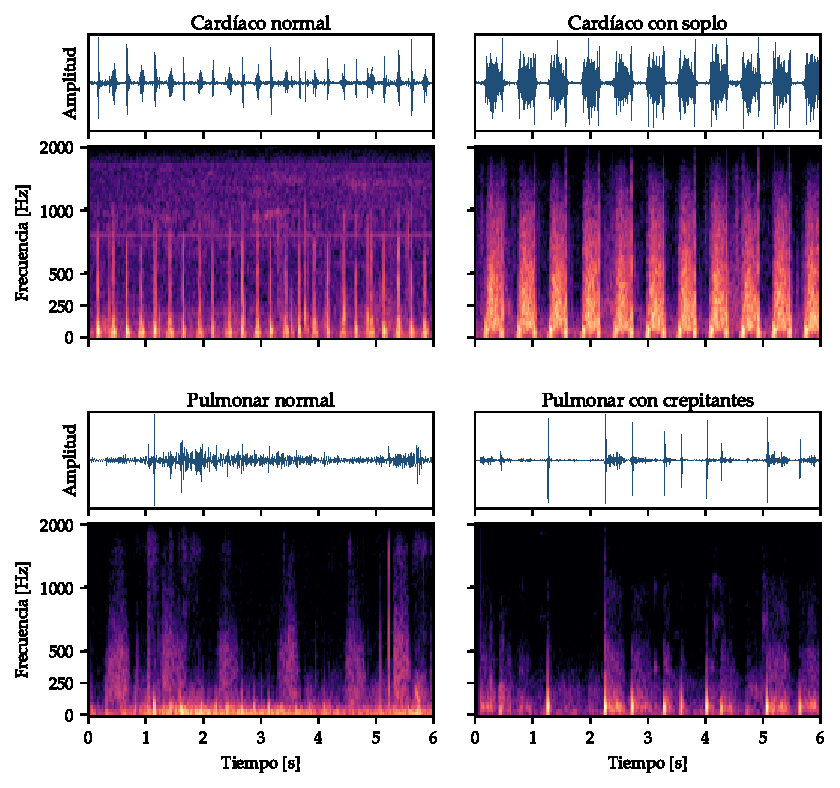
\includegraphics[width=\textwidth]{./Figures/ejemplos_auscultacion.pdf}
	\caption{Forma de onda y espectrograma en escala Mel de cuatro grabaciones de auscultación: sonido cardíaco normal, sonido cardíaco con soplo, sonido pulmonar normal y sonido pulmonar con crepitantes.}
	\label{fig:ejemplosAuscultacion}
\end{figure}

%----------------------------------------------------------------------------------------

\section{Contexto y motivación}
\label{sec:motivacion}

Las enfermedades cardiovasculares y respiratorias se encuentran entre las principales causas de muerte y de discapacidad en el mundo. Según la Organización Mundial de la Salud, en 2019 las enfermedades cardiovasculares causaron alrededor de 17,9 millones de muertes, el 32\,\% del total mundial, y más de tres cuartas partes de ellas ocurrieron en países de ingresos bajos y medios \citep{who2021cvd}. Por su parte, en 2017 se estimaba que unas 545 millones de personas vivían con alguna enfermedad respiratoria crónica, que en conjunto constituían la tercera causa de muerte a nivel mundial \citep{gbd2020chronic}. En ambos grupos de enfermedades, la detección temprana resulta determinante para el pronóstico del paciente y para reducir los costos que la enfermedad avanzada impone al sistema de salud.

El acceso a esa detección temprana no es homogéneo. En América del Sur, los profesionales de la salud se concentran en las capitales y en las grandes ciudades, mientras que las zonas rurales y desatendidas sufren faltantes que afectan de manera directa la disponibilidad de especialistas \citep{paho2026brechas}. En esos contextos, suele ser el médico generalista quien realiza la primera evaluación del paciente con el estetoscopio y quien decide, a partir de lo que escucha, si derivarlo o no a un cardiólogo o a un neumólogo. Como se señaló en la sección \ref{sec:auscultacion}, la precisión de esa evaluación depende fuertemente del entrenamiento del profesional. Un soplo o un crepitante que pasan inadvertidos pueden retrasar el diagnóstico de una enfermedad tratable. A la inversa, una derivación innecesaria consume recursos escasos.

Este escenario motiva el desarrollo de herramientas de apoyo a la decisión clínica basadas en inteligencia artificial. Un sistema capaz de analizar la señal registrada por un estetoscopio digital y de indicar la presencia de hallazgos patológicos ofrecería al médico generalista una segunda opinión objetiva y reproducible, sin reemplazar su criterio. Además, en la práctica clínica el corazón y los pulmones se auscultan durante el mismo examen, por lo que resulta de interés que una misma herramienta pueda analizar ambos tipos de sonido.

El trabajo se desarrolló en el marco de la Carrera de Especialización en Inteligencia Artificial de la Universidad de Buenos Aires, en colaboración con el Centro de Investigación y Desarrollo en Ingeniería Biomédica (CIBIO) de la Universidad Tecnológica Nacional, Facultad Regional Buenos Aires. Sus resultados son de carácter académico y de acceso abierto, para que puedan incorporarse a futuras líneas de investigación clínica del centro. Desde el punto de vista del autor, el proyecto integra su experiencia previa en procesamiento digital de señales y en desarrollos aplicados al ámbito médico con las técnicas de aprendizaje profundo estudiadas durante la especialización.

%----------------------------------------------------------------------------------------

\section{Estado del arte}
\label{sec:estadoArte}

El análisis automático de sonidos de auscultación tuvo un fuerte crecimiento durante la última década, impulsado en buena medida por la publicación de bases de datos abiertas y por desafíos científicos que permitieron comparar algoritmos bajo condiciones comunes. En el dominio cardíaco se destacan el desafío PhysioNet/Computing in Cardiology 2016, orientado a distinguir grabaciones normales de anormales \citep{clifford2016classification}, y el George B. Moody PhysioNet Challenge 2022, centrado en la detección de soplos \citep{reyna2023heart} sobre la base CirCor DigiScope, compuesta por grabaciones de pacientes pediátricos \citep{oliveira2022circor}. En el dominio pulmonar, la referencia principal es la base del desafío ICBHI 2017, con 920 grabaciones de 126 pacientes y anotaciones de crepitantes y sibilancias por ciclo respiratorio \citep{rocha2019open}. Revisiones recientes de ambos dominios muestran que el aprendizaje profundo desplazó a los métodos basados en características diseñadas manualmente \citep{ren2024comprehensive, sfayyih2023review}.

El enfoque predominante consiste en transformar la señal de audio en una representación tiempo-frecuencia, como el espectrograma en escala Mel o los coeficientes cepstrales en frecuencia Mel (MFCC, \textit{Mel-Frequency Cepstral Coefficients}), y procesarla con una red neuronal convolucional (CNN, \textit{Convolutional Neural Network}). En el desafío de 2016, la mejor propuesta combinó un clasificador basado en características con una CNN \citep{potes2016ensemble}, mientras que en el de 2022 el primer puesto en la detección de soplos correspondió a una CNN liviana que recibe el espectrograma Mel junto con datos demográficos del paciente \citep{lu2022lightweight}. En el dominio pulmonar, los trabajos más recientes incorporan transferencia de aprendizaje desde modelos preentrenados sobre grandes volúmenes de imágenes o de audio general. RespireNet adaptó una ResNet-34 preentrenada en ImageNet con técnicas de aumentación específicas para sonidos respiratorios \citep{gairola2021respirenet}, y trabajos posteriores emplearon arquitecturas basadas en \textit{transformers}, como el \textit{Audio Spectrogram Transformer}, combinadas con aprendizaje contrastivo \citep{bae2023patchmix}. La tabla \ref{tab:estadoArte} resume los trabajos más representativos.

\begin{table}[htbp]
	\centering
	\caption[Comparación de trabajos representativos del estado del arte]{Comparación de trabajos representativos en la clasificación automática de sonidos de auscultación. Se informa la métrica principal de cada trabajo sobre su conjunto de prueba; los valores no son directamente comparables entre filas porque difieren las tareas, los datos y los protocolos de partición.}
	\label{tab:estadoArte}
	\small
	\begin{tabular}{>{\raggedright\arraybackslash}p{2.0cm} >{\raggedright\arraybackslash}p{2.3cm} >{\raggedright\arraybackslash}p{2.3cm} >{\raggedright\arraybackslash}p{2.9cm} >{\raggedright\arraybackslash}p{2.1cm}}
		\toprule
		\textbf{Trabajo} & \textbf{Tarea} & \textbf{Datos} & \textbf{Modelo} & \textbf{Resultado} \\
		\midrule
		Potes et al. \citep{potes2016ensemble} & Cardíaco: normal o anormal & PhysioNet/ CinC 2016 & Ensamble de AdaBoost sobre características y CNN & Puntaje 0,860 (1.\textsuperscript{er} puesto) \\
		\addlinespace
		Lu et al. \citep{lu2022lightweight} & Cardíaco: soplo presente, ausente o desconocido & CirCor DigiScope & CNN liviana sobre espectrograma Mel y datos demográficos & Exactitud ponderada 0,780 (1.\textsuperscript{er} puesto) \\
		\addlinespace
		Gairola et al. \citep{gairola2021respirenet} & Pulmonar: 4 clases de sonidos adventicios por ciclo & ICBHI 2017 (partición oficial) & ResNet-34 preentrenada en ImageNet & Puntaje ICBHI 56,2\,\% (Se 40,1\,\%, Sp 72,3\,\%) \\
		\addlinespace
		Bae et al. \citep{bae2023patchmix} & Pulmonar: 4 clases de sonidos adventicios por ciclo & ICBHI 2017 (partición oficial) & \textit{Audio Spectrogram Transformer} con aprendizaje contrastivo & Puntaje ICBHI 62,4\,\% (Se 43,1\,\%, Sp 81,7\,\%) \\
		\addlinespace
		Tariq et al. \citep{tariq2022feature} & Pulmonar y cardíaco, con un modelo para cada dominio & ICBHI 2017 y una base pública de 656 grabaciones cardíacas & Fusión de tres CNN (espectrograma, MFCC y cromagrama) & Exactitud 99,1\,\% (pulmonar) y 97\,\% (cardíaco) \\
		\bottomrule
	\end{tabular}
\end{table}

La comparación entre trabajos debe hacerse con cautela. Cada desafío define su propia métrica: el de 2016 y el ICBHI utilizan el promedio entre sensibilidad (Se) y especificidad (Sp), mientras que el de 2022 emplea una exactitud ponderada que penaliza más los soplos no detectados. Además, la forma de particionar los datos influye fuertemente en los resultados. Sobre la partición oficial del ICBHI, los trabajos de la tabla \ref{tab:estadoArte} obtienen puntajes de entre el 56 y el 62\,\%, con sensibilidades por debajo del 45\,\%. En cambio, algunos trabajos informan exactitudes cercanas al 99\,\% con una partición 80/20 de las grabaciones, sin indicar si las grabaciones de un mismo paciente quedan separadas entre entrenamiento y prueba \citep{tariq2022feature}. Cuando esa separación no se garantiza, el modelo puede aprender características propias de cada paciente o de cada equipo de grabación, y el resultado sobreestima su desempeño ante pacientes nuevos.

Por último, la gran mayoría de los sistemas existentes aborda los sonidos cardíacos y pulmonares como dominios independientes: cada modelo se entrena con una única base de datos y reconoce solo patologías de un órgano. Incluso los trabajos que estudian ambos tipos de sonido, como el de Tariq et al., entrenan y evalúan un modelo distinto para cada dominio \citep{tariq2022feature}. Esta separación contrasta con la práctica clínica, en la que el médico ausculta el corazón y los pulmones durante un mismo examen. Recién en los últimos años aparecieron bases de datos que registran ambos sonidos de forma conjunta, como HLS-CMDS, grabada sobre un maniquí clínico \citep{torabi2025hlscmds}, lo que refleja un interés creciente por el análisis cardiopulmonar integrado. El presente trabajo se enfoca en ese vacío: abordar los sonidos cardíacos y pulmonares dentro de un mismo sistema de clasificación.

%----------------------------------------------------------------------------------------

\section{Objetivos y alcance}
\label{sec:objetivos}

% Pendiente.

\chapter{Introducción específica} % Main chapter title

\label{Chapter2}

% %----------------------------------------------------------------------------------------
% %	SECTION 1
% %----------------------------------------------------------------------------------------
% Todos los capítulos deben comenzar con un breve párrafo introductorio que indique cuál es el contenido que se encontrará al leerlo.  La redacción sobre el contenido de la memoria debe hacerse en presente y todo lo referido al proyecto en pasado, siempre de modo impersonal.

% \section{Estilo y convenciones}
% \label{sec:ejemplo}

% \subsection{Uso de mayúscula inicial para los título de secciones}

% Si en el texto se hace alusión a diferentes partes del trabajo referirse a ellas como capítulo, sección o subsección según corresponda. Por ejemplo: ``En el capítulo \ref{Chapter1} se explica tal cosa'', o ``En la sección \ref{sec:ejemplo} se presenta lo que sea'', o ``En la subsección \ref{subsec:ejemplo} se discute otra cosa''.

% Cuando se quiere poner una lista tabulada, se hace así:

% \begin{itemize}
% 	\item Este es el primer elemento de la lista.
% 	\item Este es el segundo elemento de la lista.
% \end{itemize}

% Notar el uso de las mayúsculas y el punto al final de cada elemento.

% Si se desea poner una lista numerada el formato es este:

% \begin{enumerate}
% 	\item Este es el primer elemento de la lista.
% 	\item Este es el segundo elemento de la lista.
% \end{enumerate}

% Notar el uso de las mayúsculas y el punto al final de cada elemento.

% \subsection{Este es el título de una subsección}
% \label{subsec:ejemplo}

% Se recomienda no utilizar \textbf{texto en negritas} en ningún párrafo, ni tampoco texto \underline{subrayado}. En cambio sí se debe utilizar \textit{texto en itálicas} para palabras en un idioma extranjero, al menos la primera vez que aparecen en el texto. En el caso de palabras que estamos inventando se deben utilizar ``comillas'', así como también para citas textuales. Por ejemplo, un \textit{digital filter} es una especie de ``selector'' que permite separar ciertos componentes armónicos en particular.

% La escritura debe ser impersonal. Por ejemplo, no utilizar ``el diseño del firmware lo hice de acuerdo con tal principio'', sino ``el firmware fue diseñado utilizando tal principio''. 

% El trabajo es algo que al momento de escribir la memoria se supone que ya está concluido, entonces todo lo que se refiera a hacer el trabajo se narra en tiempo pasado, porque es algo que ya ocurrió. Por ejemplo, "se diseñó el firmware empleando la técnica de test driven development".

% En cambio, la memoria es algo que está vivo cada vez que el lector la lee. Por eso transcurre siempre en tiempo presente, como por ejemplo:

% ``En el presente capítulo se da una visión global sobre las distintas pruebas realizadas y los resultados obtenidos. Se explica el modo en que fueron llevados a cabo los test unitarios y las pruebas del sistema''.

% Se recomienda no utilizar una sección de glosario sino colocar la descripción de las abreviaturas como parte del mismo cuerpo del texto. Por ejemplo, RTOS (\textit{Real Time Operating System}, Sistema Operativo de Tiempo Real) o en caso de considerarlo apropiado mediante notas a pie de página.

% Si se desea indicar alguna página web utilizar el siguiente formato de referencias bibliográficas, dónde las referencias se detallan en la sección de bibliografía de la memoria, utilizado el formato establecido por IEEE en \citep{IEEE:citation}. Por ejemplo, ``el presente trabajo se basa en la plataforma EDU-CIAA-NXP \citep{CIAA}, la cual...''.

% \subsection{Figuras} 

% Al insertar figuras en la memoria se deben considerar determinadas pautas. Para empezar, usar siempre tipografía claramente legible. Luego, tener claro que \textbf{es incorrecto} escribir por ejemplo esto: ``El diseño elegido es un cuadrado, como se ve en la siguiente figura:''

% \begin{figure}[h]
% \centering
% 
\includegraphics[scale=.45]{./Figures/cuadradoAzul.png}
% \end{figure}

% La forma correcta de utilizar una figura es con referencias cruzadas, por ejemplo: ``Se eligió utilizar un cuadrado azul para el logo, como puede observarse en la figura \ref{fig:cuadradoAzul}''.

% \begin{figure}[ht]
% 	\centering
% 	
\includegraphics[scale=.45]{./Figures/cuadradoAzul.png}
% 	\caption{Ilustración del cuadrado azul que se eligió para el diseño del logo.}
% 	\label{fig:cuadradoAzul}
% \end{figure}

% El texto de las figuras debe estar siempre en español, excepto que se decida reproducir una figura original tomada de alguna referencia. En ese caso la referencia de la cual se tomó la figura debe ser indicada en el epígrafe de la figura e incluida como una nota al pie, como se ilustra en la figura \ref{fig:palabraIngles}.

% \begin{figure}[htpb]
% 	\centering
% 	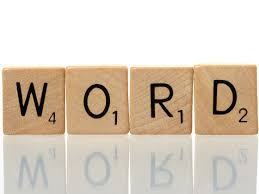
\includegraphics[scale=.3]{./Figures/word.jpeg}
% 	\caption{Imagen tomada de la página oficial del procesador\protect\footnotemark.}
% 	\label{fig:palabraIngles}
% \end{figure}

% \footnotetext{Imagen tomada de \url{https://goo.gl/images/i7C70w}}

% La figura y el epígrafe deben conformar una unidad cuyo significado principal pueda ser comprendido por el lector sin necesidad de leer el cuerpo central de la memoria. Para eso es necesario que el epígrafe sea todo lo detallado que corresponda y si en la figura se utilizan abreviaturas entonces aclarar su significado en el epígrafe o en la misma figura.



% \begin{figure}[ht]
% 	\centering
% 	
\includegraphics[scale=.37]{./Figures/questionMark.png}
% 	\caption{¿Por qué de pronto aparece esta figura?}
% 	\label{fig:questionMark}
% \end{figure}

% Nunca colocar una figura en el documento antes de hacer la primera referencia a ella, como se ilustra con la figura \ref{fig:questionMark}, porque sino el lector no comprenderá por qué de pronto aparece la figura en el documento, lo que distraerá su atención.

% Otra posibilidad es utilizar el entorno \textit{subfigure} para incluir más de una figura, como se puede ver en la figura \ref{fig:three graphs}. Notar que se pueden referenciar también las figuras internas individualmente de esta manera: \ref{fig:1de3}, \ref{fig:2de3} y \ref{fig:3de3}.
 
% \begin{figure}[!htpb]
%      \centering
%      \begin{subfigure}[b]{0.3\textwidth}
%          \centering
%          
\includegraphics[width=.65\textwidth]{./Figures/questionMark}
%          \caption{Un caption.}
%          \label{fig:1de3}
%      \end{subfigure}
%      \hfill
%      \begin{subfigure}[b]{0.3\textwidth}
%          \centering
%          
\includegraphics[width=.65\textwidth]{./Figures/questionMark}
%          \caption{Otro.}
%          \label{fig:2de3}
%      \end{subfigure}
%      \hfill
%      \begin{subfigure}[b]{0.3\textwidth}
%          \centering
%          
\includegraphics[width=.65\textwidth]{./Figures/questionMark}
%          \caption{Y otro más.}
%          \label{fig:3de3}
%      \end{subfigure}
%         \caption{Tres gráficos simples.}
%         \label{fig:three graphs}
% \end{figure}

% El código para generar las imágenes se encuentra disponible para su reutilización en el archivo \file{Chapter2.tex}.

% \subsection{Tablas}

% Para las tablas utilizar el mismo formato que para las figuras, sólo que el epígrafe se debe colocar arriba de la tabla, como se ilustra en la tabla \ref{tab:peces}. Observar que sólo algunas filas van con líneas visibles y notar el uso de las negritas para los encabezados.  La referencia se logra utilizando el comando \verb|\ref{<label>}| donde label debe estar definida dentro del entorno de la tabla.

% \begin{verbatim}
% \begin{table}[h]
% 	\centering
% 	\caption[caption corto]{caption largo más descriptivo}
% 	\begin{tabular}{l c c}    
% 		\toprule
% 		\textbf{Especie}     & \textbf{Tamaño} & \textbf{Valor}\\
% 		\midrule
% 		Amphiprion Ocellaris & 10 cm           & \$ 6.000 \\		
% 		Hepatus Blue Tang    & 15 cm           & \$ 7.000 \\
% 		Zebrasoma Xanthurus  & 12 cm           & \$ 6.800 \\
% 		\bottomrule
% 		\hline
% 	\end{tabular}
% 	\label{tab:peces}
% \end{table}
% \end{verbatim}


% \begin{table}[h]
% 	\centering
% 	\caption[caption corto]{caption largo más descriptivo.}
% 	\begin{tabular}{l c c}    
% 		\toprule
% 		\textbf{Especie} 	 & \textbf{Tamaño} 		& \textbf{Valor}  \\
% 		\midrule
% 		Amphiprion Ocellaris & 10 cm 				& \$ 6.000 \\		
% 		Hepatus Blue Tang	 & 15 cm				& \$ 7.000 \\
% 		Zebrasoma Xanthurus	 & 12 cm				& \$ 6.800 \\
% 		\bottomrule
% 		\hline
% 	\end{tabular}
% 	\label{tab:peces}
% \end{table}

% En cada capítulo se debe reiniciar el número de conteo de las figuras y las tablas, por ejemplo, figura 2.1 o tabla 2.1, pero no se debe reiniciar el conteo en cada sección. Por suerte la plantilla se encarga de esto por nosotros.

% \subsection{Ecuaciones}
% \label{sec:Ecuaciones}

% Al insertar ecuaciones en la memoria dentro de un entorno \textit{equation}, éstas se numeran en forma automática  y se pueden referir al igual que como se hace con las figuras y tablas, por ejemplo ver la ecuación \ref{eq:metric}.

% \begin{equation}
% 	\label{eq:metric}
% 	ds^2 = c^2 dt^2 \left( \frac{d\sigma^2}{1-k\sigma^2} + \sigma^2\left[ d\theta^2 + \sin^2\theta d\phi^2 \right] \right)
% \end{equation}
                                                        
% Para generar la ecuación \ref{eq:metric} se utilizó el siguiente código:

% \begin{verbatim}
% \begin{equation}
% 	\label{eq:metric}
% 	ds^2 = c^2 dt^2 \left( \frac{d\sigma^2}{1-k\sigma^2} + 
% 	\sigma^2\left[ d\theta^2 + 
% 	\sin^2\theta d\phi^2 \right] \right)
% \end{equation}
% \end{verbatim}

\chapter{Diseño e implementación} % Main chapter title

\label{Chapter3} % Change X to a consecutive number; for referencing this chapter elsewhere, use \ref{ChapterX}

% Todos los capítulos deben comenzar con un breve párrafo introductorio que indique cuál es el contenido que se encontrará al leerlo.  La redacción sobre el contenido de la memoria debe hacerse en presente y todo lo referido al proyecto en pasado, siempre de modo impersonal.

% \definecolor{mygreen}{rgb}{0,0.6,0}
% \definecolor{mygray}{rgb}{0.5,0.5,0.5}
% \definecolor{mymauve}{rgb}{0.58,0,0.82}

% %%%%%%%%%%%%%%%%%%%%%%%%%%%%%%%%%%%%%%%%%%%%%%%%%%%%%%%%%%%%%%%%%%%%%%%%%%%%%
% % parámetros para configurar el formato del código en los entornos lstlisting
% %%%%%%%%%%%%%%%%%%%%%%%%%%%%%%%%%%%%%%%%%%%%%%%%%%%%%%%%%%%%%%%%%%%%%%%%%%%%%
% \lstset{ %
%   backgroundcolor=\color{white},   % choose the background color; you must add \usepackage{color} or \usepackage{xcolor}
%   basicstyle=\footnotesize,        % the size of the fonts that are used for the code
%   breakatwhitespace=false,         % sets if automatic breaks should only happen at whitespace
%   breaklines=true,                 % sets automatic line breaking
%   captionpos=b,                    % sets the caption-position to bottom
%   commentstyle=\color{mygreen},    % comment style
%   deletekeywords={...},            % if you want to delete keywords from the given language
%   %escapeinside={\%*}{*)},          % if you want to add LaTeX within your code
%   %extendedchars=true,              % lets you use non-ASCII characters; for 8-bits encodings only, does not work with UTF-8
%   %frame=single,	                % adds a frame around the code
%   keepspaces=true,                 % keeps spaces in text, useful for keeping indentation of code (possibly needs columns=flexible)
%   keywordstyle=\color{blue},       % keyword style
%   language=[ANSI]C,                % the language of the code
%   %otherkeywords={*,...},           % if you want to add more keywords to the set
%   numbers=left,                    % where to put the line-numbers; possible values are (none, left, right)
%   numbersep=5pt,                   % how far the line-numbers are from the code
%   numberstyle=\tiny\color{mygray}, % the style that is used for the line-numbers
%   rulecolor=\color{black},         % if not set, the frame-color may be changed on line-breaks within not-black text (e.g. comments (green here))
%   showspaces=false,                % show spaces everywhere adding particular underscores; it overrides 'showstringspaces'
%   showstringspaces=false,          % underline spaces within strings only
%   showtabs=false,                  % show tabs within strings adding particular underscores
%   stepnumber=1,                    % the step between two line-numbers. If it's 1, each line will be numbered
%   stringstyle=\color{mymauve},     % string literal style
%   tabsize=2,	                   % sets default tabsize to 2 spaces
%   title=\lstname,                  % show the filename of files included with \lstinputlisting; also try caption instead of title
%   morecomment=[s]{/*}{*/}
% }


% %----------------------------------------------------------------------------------------
% %	SECTION 1
% %----------------------------------------------------------------------------------------
% \section{Análisis del software}
 
% La idea de esta sección es resaltar los problemas encontrados, los criterios utilizados y la justificación de las decisiones que se hayan tomado.

% Se puede agregar código o pseudocódigo dentro de un entorno lstlisting con el siguiente código:

% \begin{verbatim}
% \begin{lstlisting}[caption= "un epígrafe descriptivo"]
% 	las líneas de código irían aquí...
% \end{lstlisting}
% \end{verbatim}

% A modo de ejemplo, se muestra el fragmento de código \ref{cod:vControl}:

% \begin{lstlisting}[label=cod:vControl,caption=Pseudocódigo del lazo principal de control.]  % Start your code-block

% #define MAX_SENSOR_NUMBER 3
% #define MAX_ALARM_NUMBER  6
% #define MAX_ACTUATOR_NUMBER 6

% uint32_t sensorValue[MAX_SENSOR_NUMBER];		
% FunctionalState alarmControl[MAX_ALARM_NUMBER];	//ENABLE or DISABLE
% state_t alarmState[MAX_ALARM_NUMBER];						//ON or OFF
% state_t actuatorState[MAX_ACTUATOR_NUMBER];			//ON or OFF

% void vControl() {

% 	initGlobalVariables();
	
% 	period = 500 ms;
		
% 	while(1) {

% 		ticks = xTaskGetTickCount();
		
% 		updateSensors();
		
% 		updateAlarms();
		
% 		controlActuators();
		
% 		vTaskDelayUntil(&ticks, period);
% 	}
% }
% \end{lstlisting}




% Chapter Template

\chapter{Ensayos y resultados} % Main chapter title

\label{Chapter4} % Change X to a consecutive number; for referencing this chapter elsewhere, use \ref{ChapterX}
% Todos los capítulos deben comenzar con un breve párrafo introductorio que indique cuál es el contenido que se encontrará al leerlo.  La redacción sobre el contenido de la memoria debe hacerse en presente y todo lo referido al proyecto en pasado, siempre de modo impersonal.

% %----------------------------------------------------------------------------------------
% %	SECTION 1
% %----------------------------------------------------------------------------------------

% \section{Pruebas funcionales del hardware}
% \label{sec:pruebasHW}

% La idea de esta sección es explicar cómo se hicieron los ensayos, qué resultados se obtuvieron y analizarlos.

% Chapter Template

\chapter{Conclusiones} % Main chapter title

\label{Chapter5} % Change X to a consecutive number; for referencing this chapter elsewhere, use \ref{ChapterX}
% Todos los capítulos deben comenzar con un breve párrafo introductorio que indique cuál es el contenido que se encontrará al leerlo.  La redacción sobre el contenido de la memoria debe hacerse en presente y todo lo referido al proyecto en pasado, siempre de modo impersonal.


% %----------------------------------------------------------------------------------------

% %----------------------------------------------------------------------------------------
% %	SECTION 1
% %----------------------------------------------------------------------------------------

% \section{Conclusiones generales }

% La idea de esta sección es resaltar cuáles son los principales aportes del trabajo realizado y cómo se podría continuar. Debe ser especialmente breve y concisa. Es buena idea usar un listado para enumerar los logros obtenidos.

% En esta sección no se deben incluir ni tablas ni gráficos.

% Algunas preguntas que pueden servir para completar este capítulo:

% \begin{itemize}
% \item ¿Cuál es el grado de cumplimiento de los requerimientos?
% \item ¿Cuán fielmente se puedo seguir la planificación original (cronograma incluido)?
% \item ¿Se manifestó algunos de los riesgos identificados en la planificación? ¿Fue efectivo el plan de mitigación? ¿Se debió aplicar alguna otra acción no contemplada previamente?
% \item Si se debieron hacer modificaciones a lo planificado ¿Cuáles fueron las causas y los efectos?
% \item ¿Qué técnicas resultaron útiles para el desarrollo del proyecto y cuáles no tanto?
% \end{itemize}


% %----------------------------------------------------------------------------------------
% %	SECTION 2
% %----------------------------------------------------------------------------------------
% \section{Próximos pasos}

% Acá se indica cómo se podría continuar el trabajo más adelante.


%----------------------------------------------------------------------------------------
% Apéndices
%----------------------------------------------------------------------------------------

\appendix

% Incluir apéndices desde archivos separados si es necesario
%% Appendix A

\chapter{Appendix Title Here} % Main appendix title

\label{AppendixA} % For referencing this appendix elsewhere, use \ref{AppendixA}

Write your Appendix content here.

%----------------------------------------------------------------------------------------
% Bibliografía
%----------------------------------------------------------------------------------------

\renewcommand{\bibname}{Bibliografía} % Para asegurarte de que el título sea correcto
\phantomsection % Necesario para que el enlace del marcador sea correcto

\printbibliography[heading=bibintoc]

\end{document}






